\documentclass{article}
\usepackage[font=small,labelfont=bf]{caption}
\usepackage[utf8]{inputenc}
\usepackage{amsthm}
\usepackage{graphicx}
\usepackage{hyperref}
\usepackage{pdfpages}
\begin{document}

\begin{titlepage}
    \begin{center}
        \vspace*{1cm}
            
        \Huge
        \textbf{Lab 9 Report}
            
        \vspace{0.5cm}
        \LARGE
        Analysis of the Chemical Composition of Various Cannabis Products
            
        \vspace{1.5cm}
            
        \textbf{Wenqi Guo*}, Austin and Mathew
        \begin{small}
            \url{https://scholar.google.com/citations?user=4YWcPZoAAAAJ}
        \end{small}

            
        \vfill
            
TA name:
Adebowale, Adeyemi 

            
        \vspace{0.8cm}
            

            
        \Large
        Department of Chemistry\\
        University of British Columbia\\
        Dec 13, 2022
            
    \end{center}
\end{titlepage}
Code and raw \LaTeX \; of this lab report can be found on \url{https://github.com/weathon/Chem-Lab-9}
\section*{Abstract}

Cannabis markets are increasing \cite{Lab Manuel} in both Canada and the US.   In this paper, we analyzed the data set from the publication  \cite{dataset1} and \cite{dataset2} using various methods. This dataset contains the composition of 12 cannabis strains using HPLC-UV. \cite{Lab Manuel, dataset1, dataset2} We first did an ANOVA of different substances in different strains. 
We then used metaboanalyst.ca to do the Pearson Correlation on the dataset. Then we used Python to analyze the dataset using PCA and SAM. In ANOVA, most of the tests show a p-value less than 0.05,  We find that THCA contributed a lot for loading 1 and CMPD4 (this is an unknown) contributed a lot for Loading 2 in PCA. In the correlation analysis, we find that there are a few substances that are positively correlated to others, and we find no string of negative correlations in this analysis. This means these 2 compounds are important in cluster cannabis. 


\textbf{Keywords: } Cannabis, Statistical Analysis, Dataset, Significance Analysis of Microarrays, Principal Component Analysis
\newpageye
\section{Introduction}
Cannabis markets are increasing \cite{Lab Manuel} in both Canada and the US. The legal market in North America in 2021 is USD 12.4 billion, and this is rising. \cite{Market} Thus, understanding the composition of these is important for health professionals, governments, and consumers. HPLC (High-Performance Liquid Chromoptaphhy) is a method used to separate mixtures, and UV detection is commonly used to detect the  substances from HPLC in time serials. This data can then be converted to the concentration of each substance in the original sample. The correlation matrix is a method used to analyze if there are linear correlations between variables between a set of variables. PCA was commonly used to reduce the dimension of the data while keeping as much information as possible. It uses the singular vectors of the matrix. \cite{PCA} In a set of information, the higher the entropy, the more information it has. \cite{info} In the dataset, the higher the variance, the more information it contains. PCA is a linear transformation, by which the data scaler projection with the greatest variance will lie on the first dimension. \cite{PCA} In this paper, we analyzed the data using ANOVA, Coorelatonn, PCA (Principal Component Analysis), and SAM (Significance Analysis of Microarrays) \cite{SAM} on a dataset containing substances from 12 cannabis strains using HPLC-UV. \cite{dataset1} and \cite{dataset2}. \\
Understanding the substances in cannabis is important for the government to make policies, for consumers to understand the potential health effects, and for medical workers and researchers to understand the public health related to cannabis products. In this paper, we will process the data and find out if each substance is present in different amounts in different classes of cannabis, if some substances are present along with other substances, and if some will inhibit the presence of other substances, cluster different class using PCA, and "to reduce data complexity and identify key metabolites that are significant in sample classification." \cite{Lab Manuel}


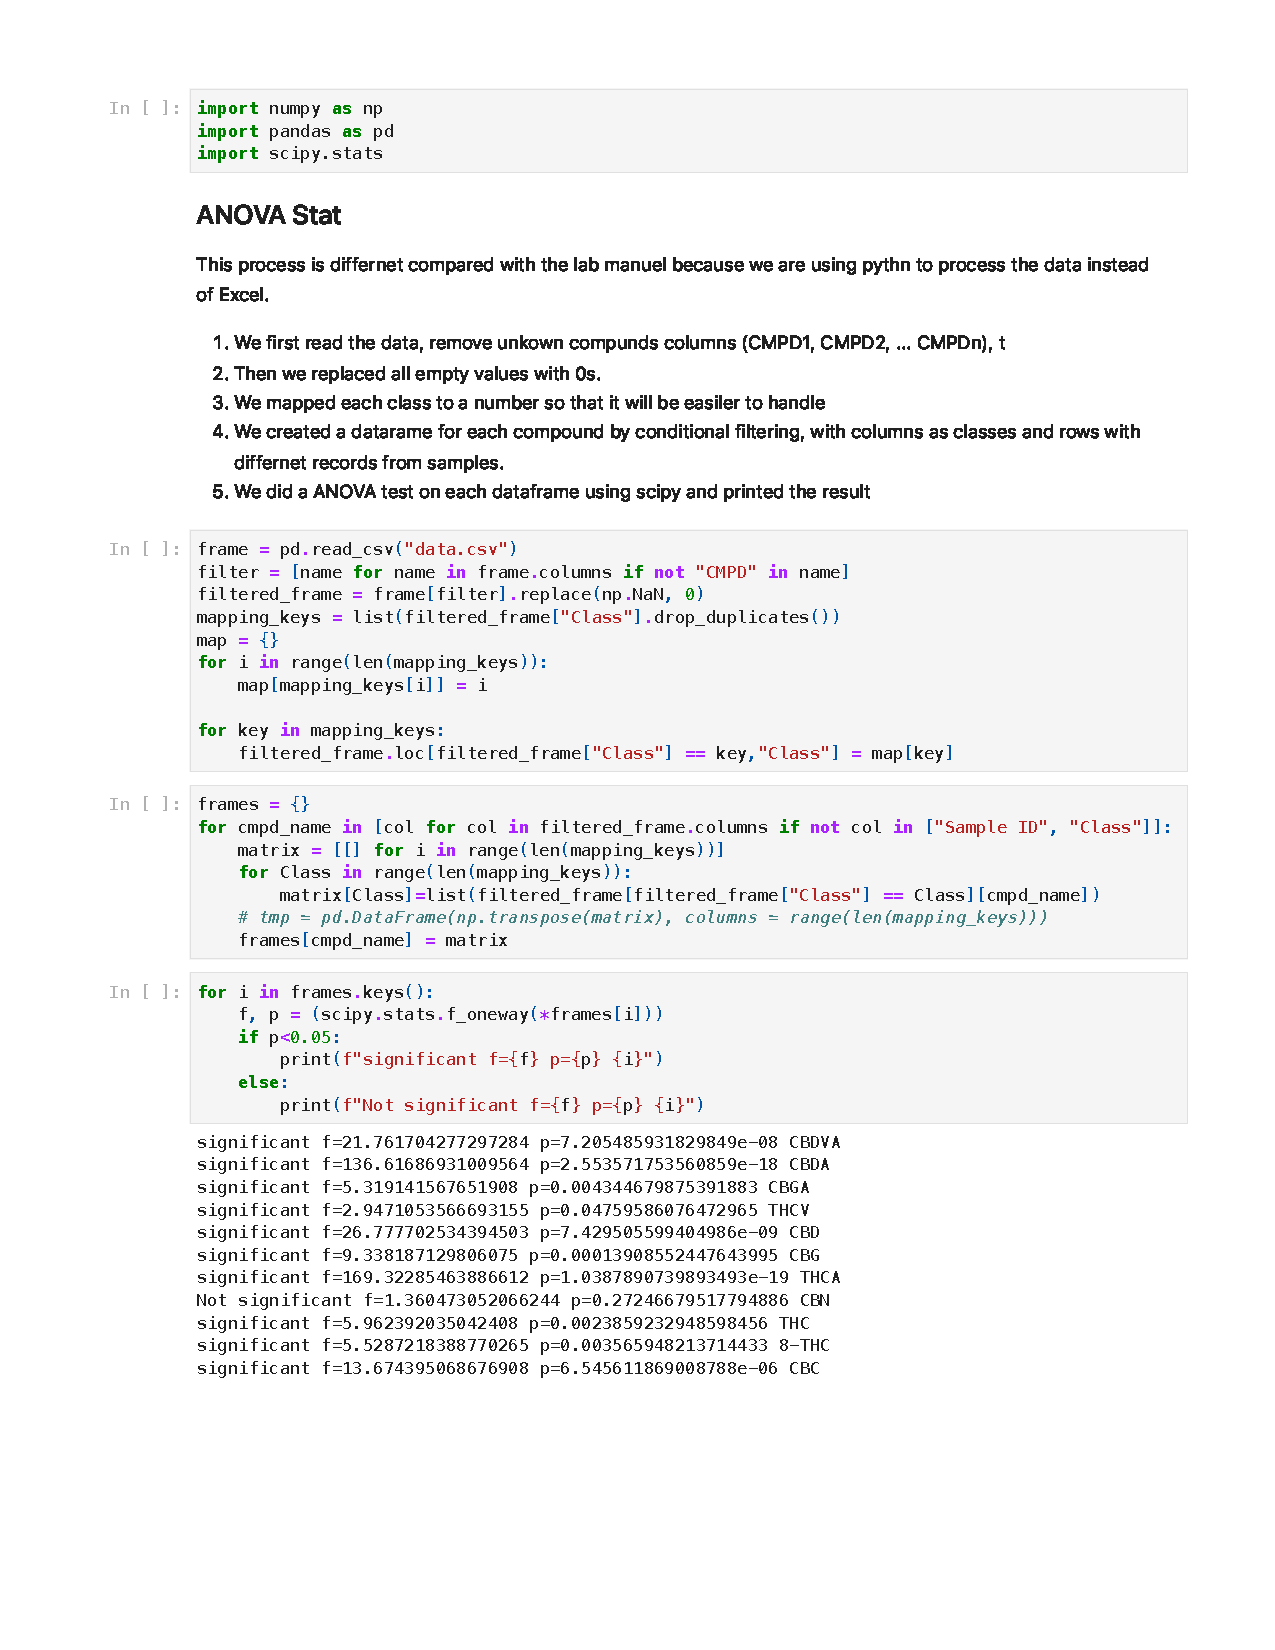
\includepdf[scale=0.8, offset=0 -2cm, pagecommand=\section{Materials and Methods} These process are based on \cite{Lab Manuel}. We converted the Excel file into a CSV file.]{main.pdf}
\subsection*{MaetaboanAlyst}
We used MetaboanAlyst for the rest of the data analytics.  We used the same dataset as we did in the last section. 


\begin{enumerate}
    \item We uploaded the CSV file to AetaboanAlyst with one var statistical analytics with the data type of concentration and sample of "rows (unpaired)." 
    \item We then skipped the missing value filling.
    \item We then normalized the data with "auto-scaling"
    \item In the statistical analysis model, we selected correlation. Then the website crashed. When I tried to reconnect, it said connection refused. It did go back for a while, but because of the unstableness, we moved on to using Python to do these analytics. 
    \item We load the data into the Pandas data frame, since correlation is independent then normalization, we don't need to normalize our data in this step.
    % then we calculate the mean and standard deviation, using which we normalized the data. 
    \item We replaced all missing values with 0s and removed all columns with only 0
    \item We got the correlation matrix using the built-in function as shown in \cite{pandaCo}, and we plotted the matrix using a heat map, as shown in figure 1.
    \item We then highlighted the substances with high correlation ($p>0.8$ for positive correlation and $p<0.8$ for negative correlation), as shown in figure 2.
    
    % and got the following
    % 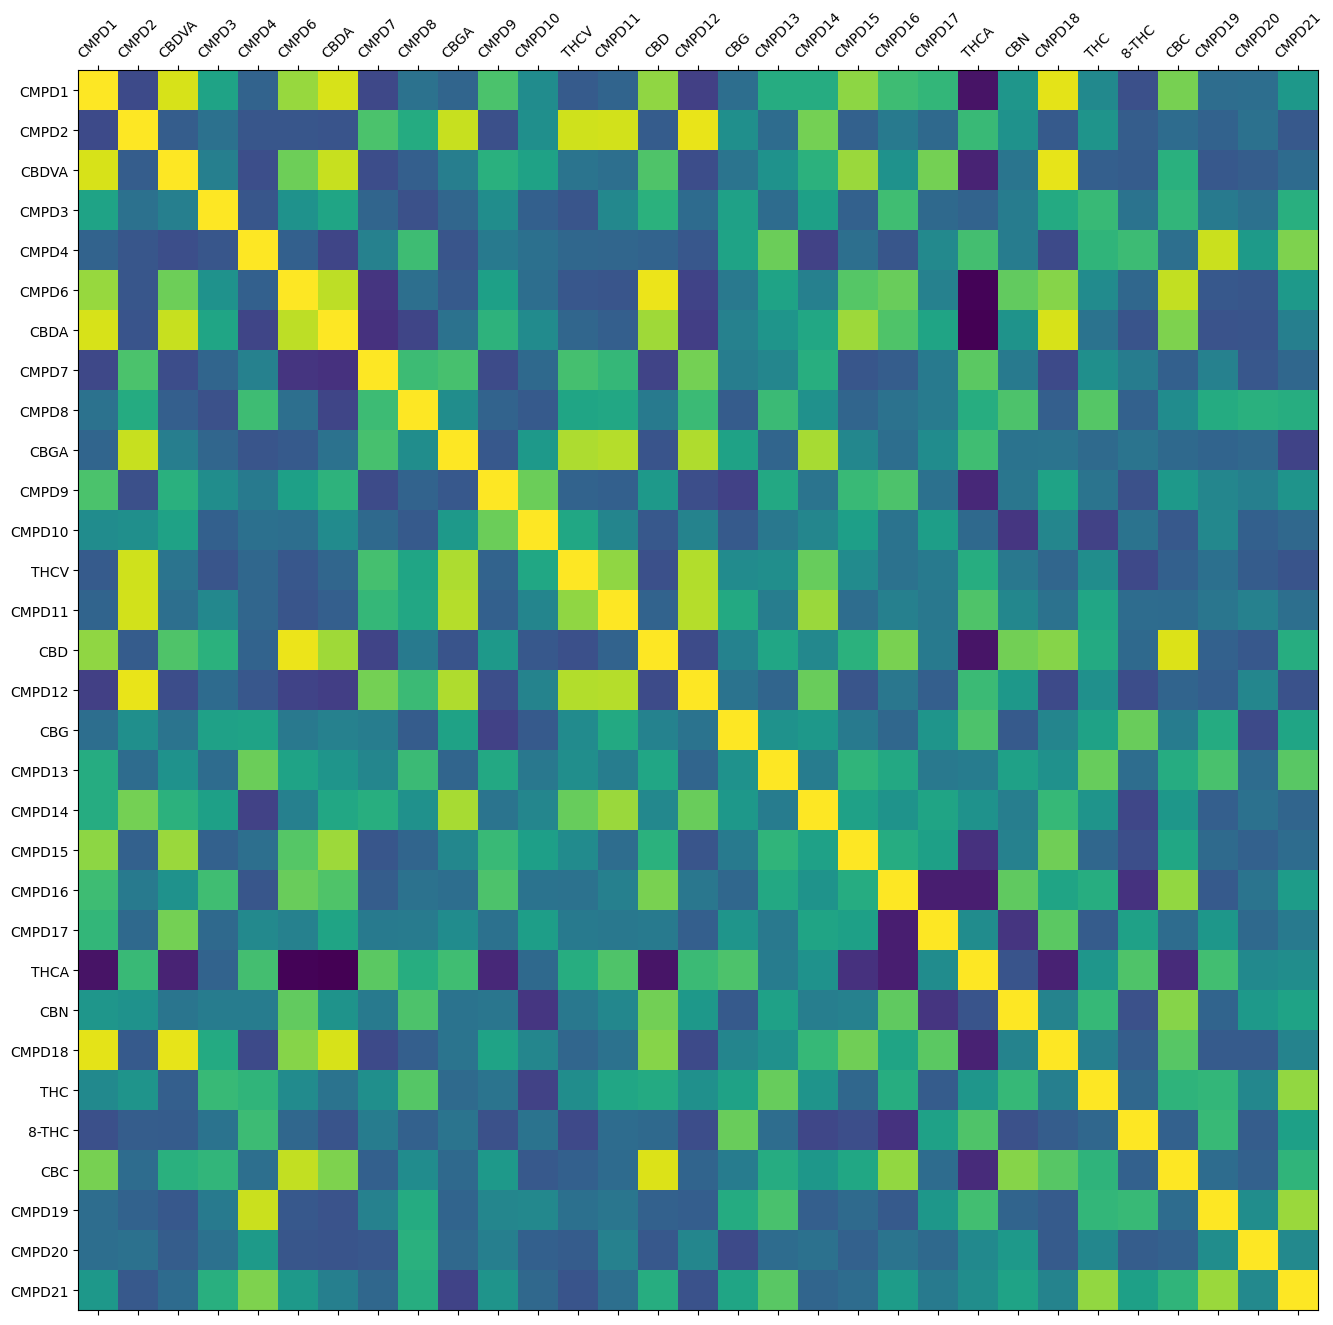
\includegraphics[scale=0.20]{output.png}
    % \item We removed all NaN values, 
    % \item Thus, we moved on to using Python to do these analytics. 
\end{enumerate}

\subsection*{Principal Component Analysis}
(The website is working again, so this part is done using the website)
\begin{enumerate}
    \item We normalized the data, then in the stat section, we selected PCA with 2 PC.
    \item We generated the 2D Scores Plot (Fig 3) and loading plot (Fig 4)
    \item We downloaded the loading data as CSV and then plotted 2 bar plots using Python. (Fig 5 and 6)
    \item We then analyze the plots and analyzing is in the Result section. 
\end{enumerate}


\subsection*{SAM}
\begin{enumerate}
    \item We selected the SAM in the stat section
    \item We increased the delta value so that the False number is 0
    \item We saved the figure as Fig 6
    \item We then downloaded the CSV file of significant metabolites
    \item We compared the result from SAM with ANOVA, the analysis is in the Result section
\end{enumerate}

\subsection*{Envirement for The code} 
All the code was finished on getpod.io using the following parameter:
\begin{itemize}
    \item Python 3.8.13 [GCC 9.4.0] on Linux
    \item NumPy 1.23.5
    \item Pandas 1.5.2
    \item Matplotlib 3.6.2
\end{itemize}

\section{Result}

\centering
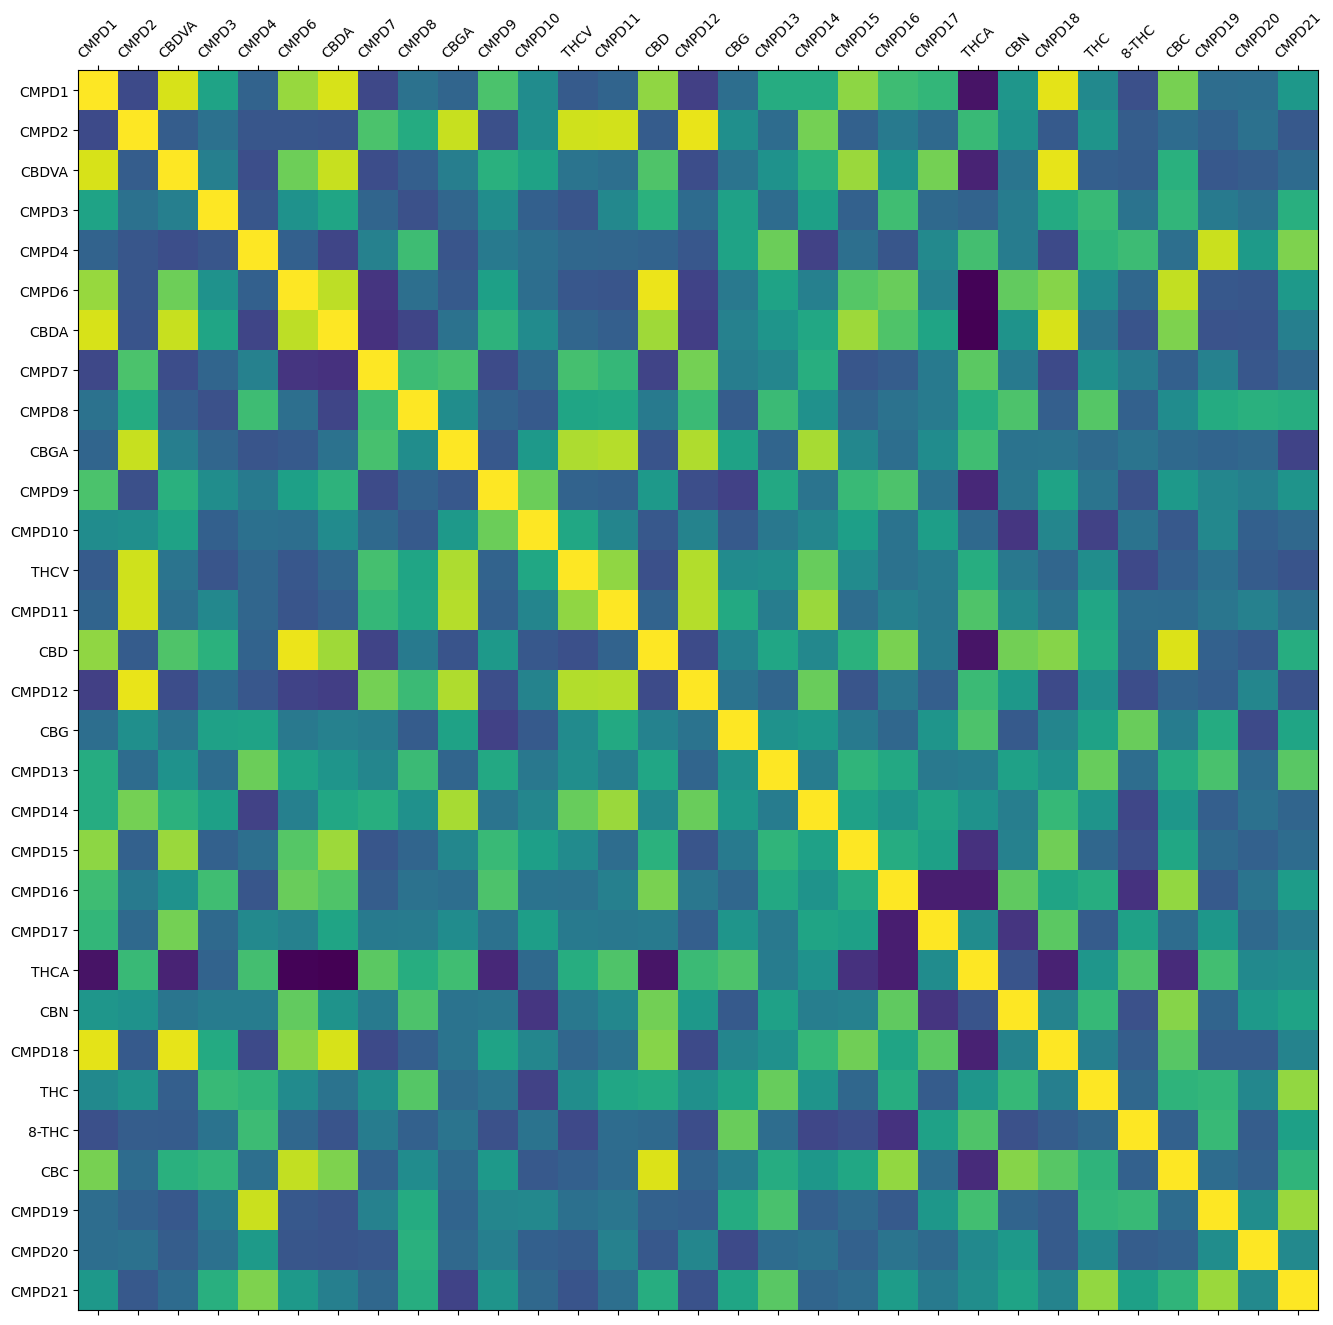
\includegraphics[width=0.7\textwidth]{output.png}
\captionof{figure}{Correlation plot of all substances}

% We can see that THCA contributed a lot for loading 1 and CMPD4 (this is an unknown) contributed a lot for Loading 2. 

% We compared that 
\\
\centering
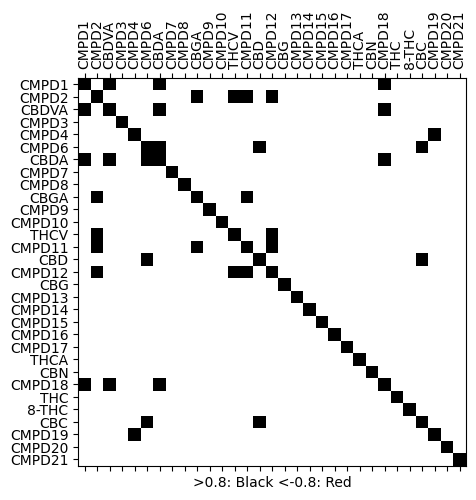
\includegraphics[width=0.7\textwidth]{output2.png}
\captionof{figure}{Figure 2. Correlation plot of all substances with $>0.8$ or $<-0.8$ highlighted}

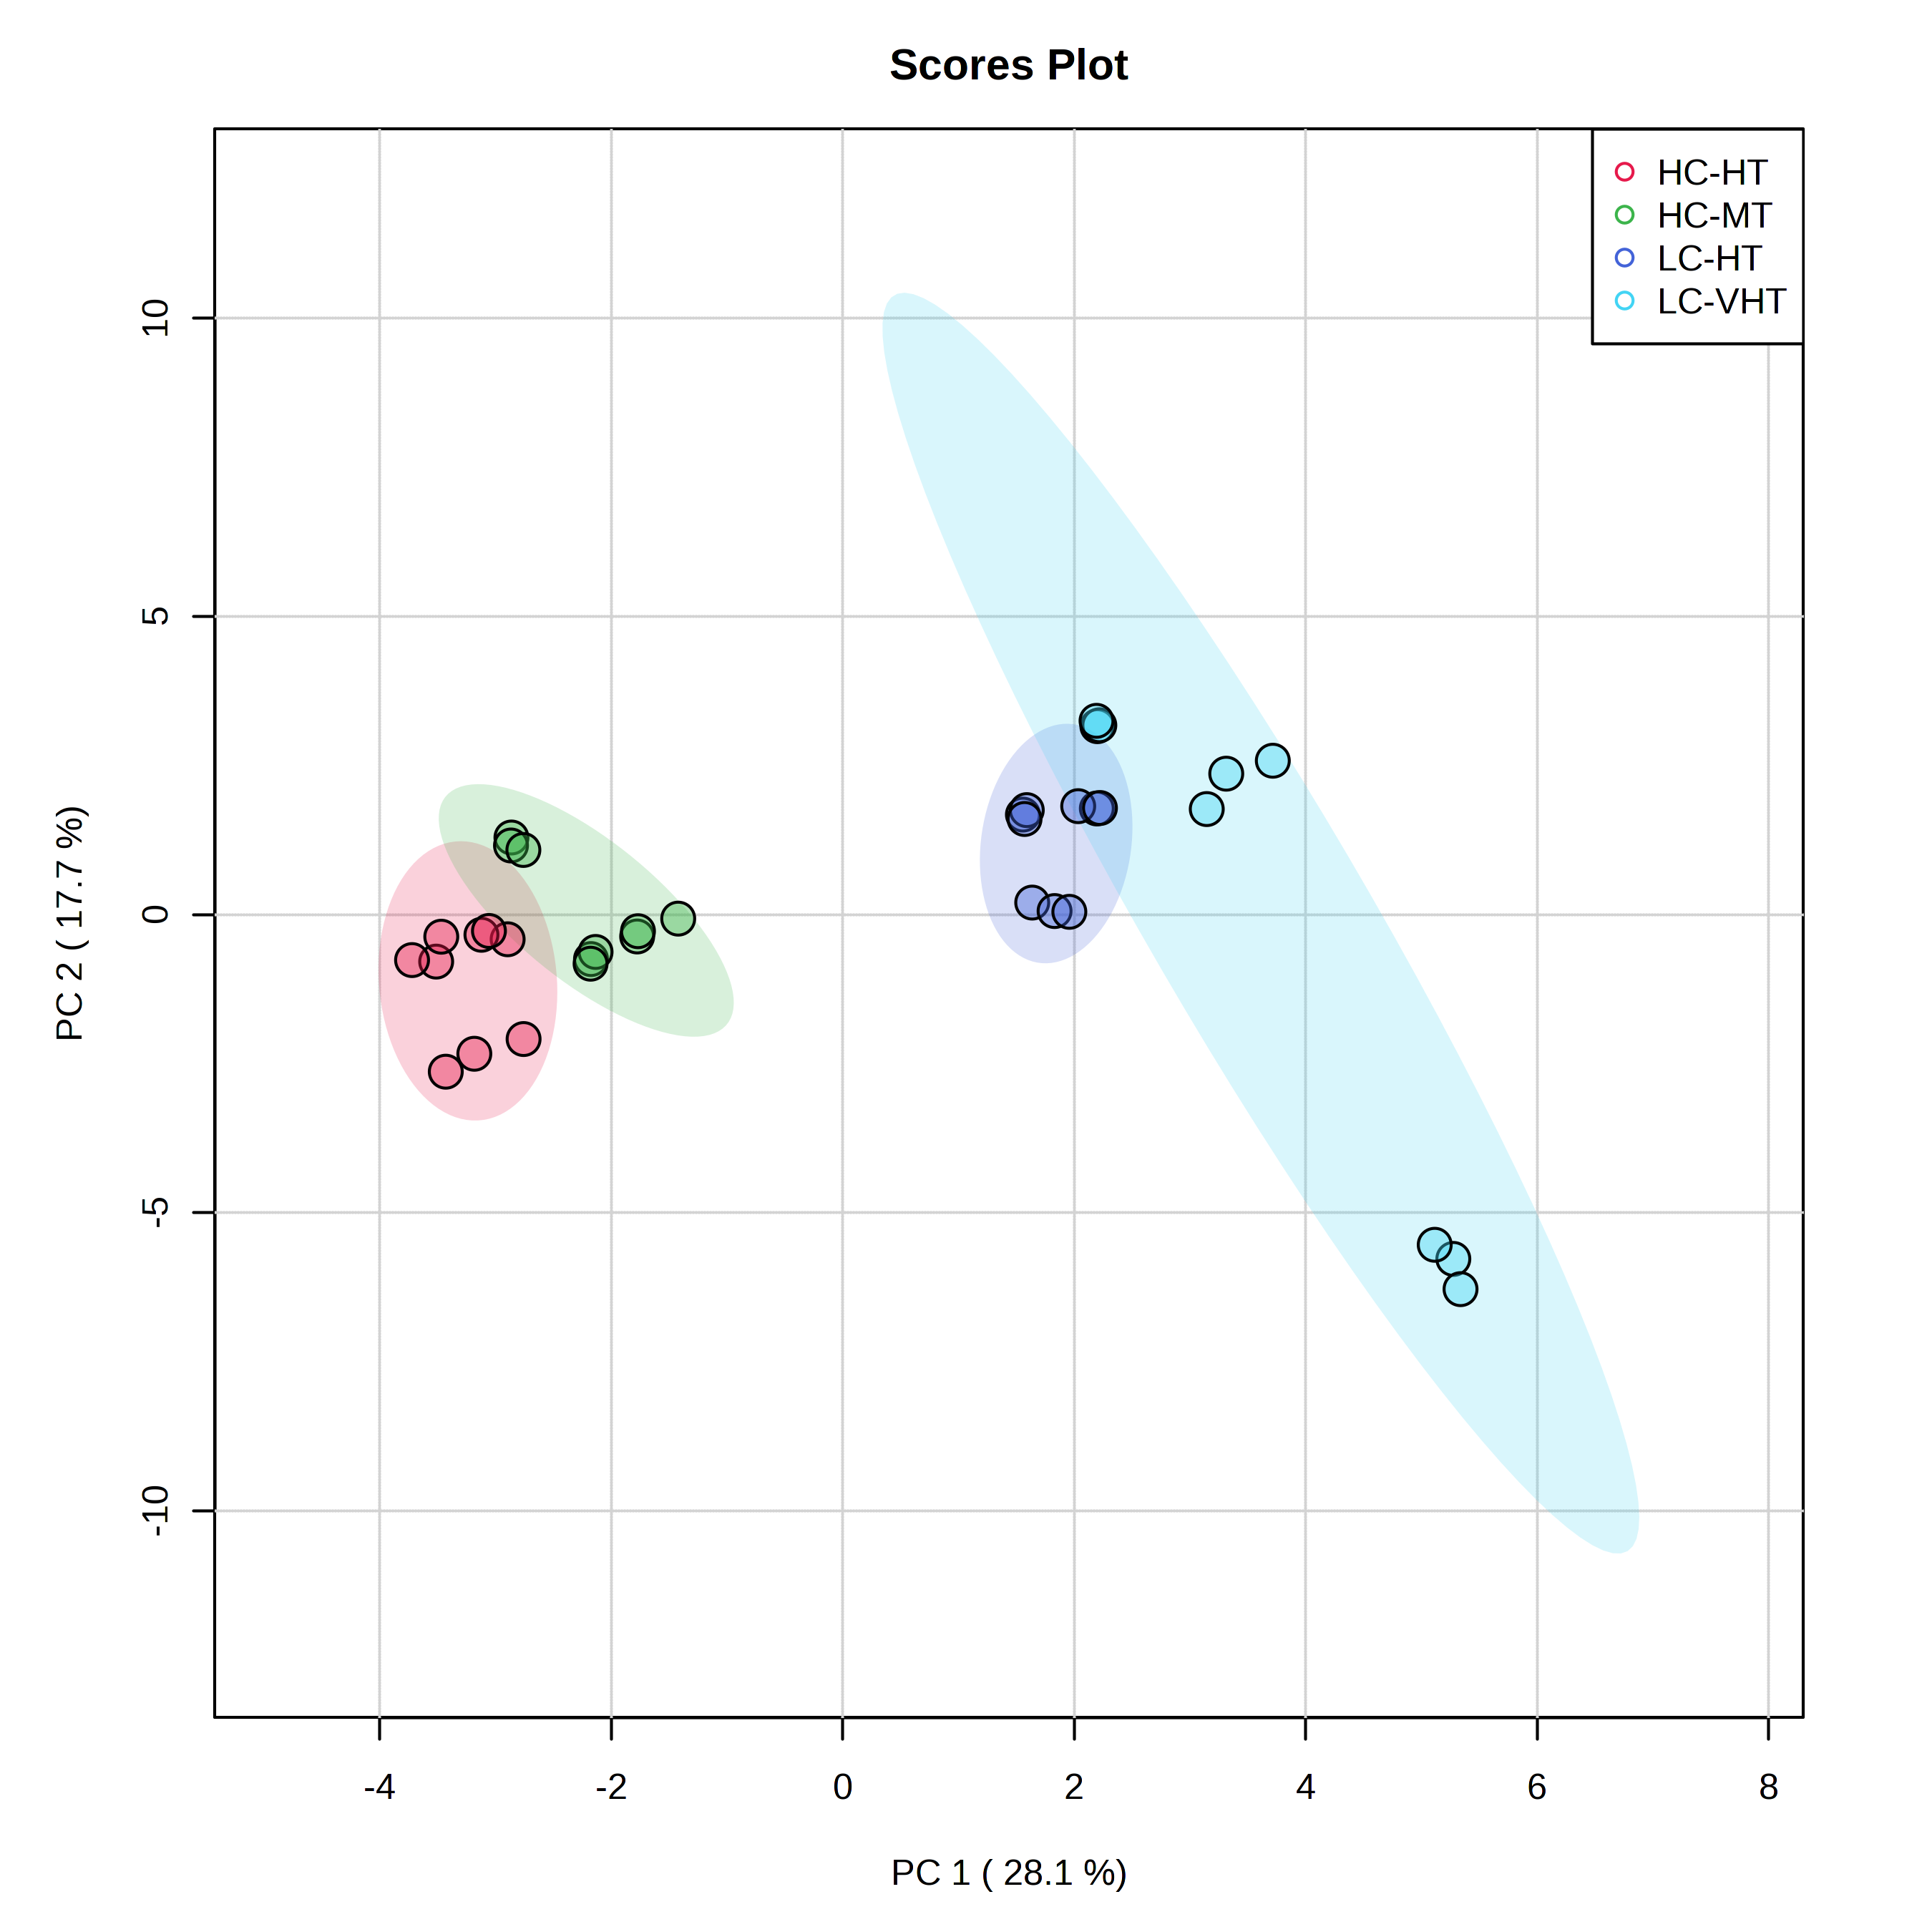
\includegraphics[width=0.7\textwidth]{pca_score2d_1_dpi300.png}
\captionof{figure}{ PCA Score Plot}

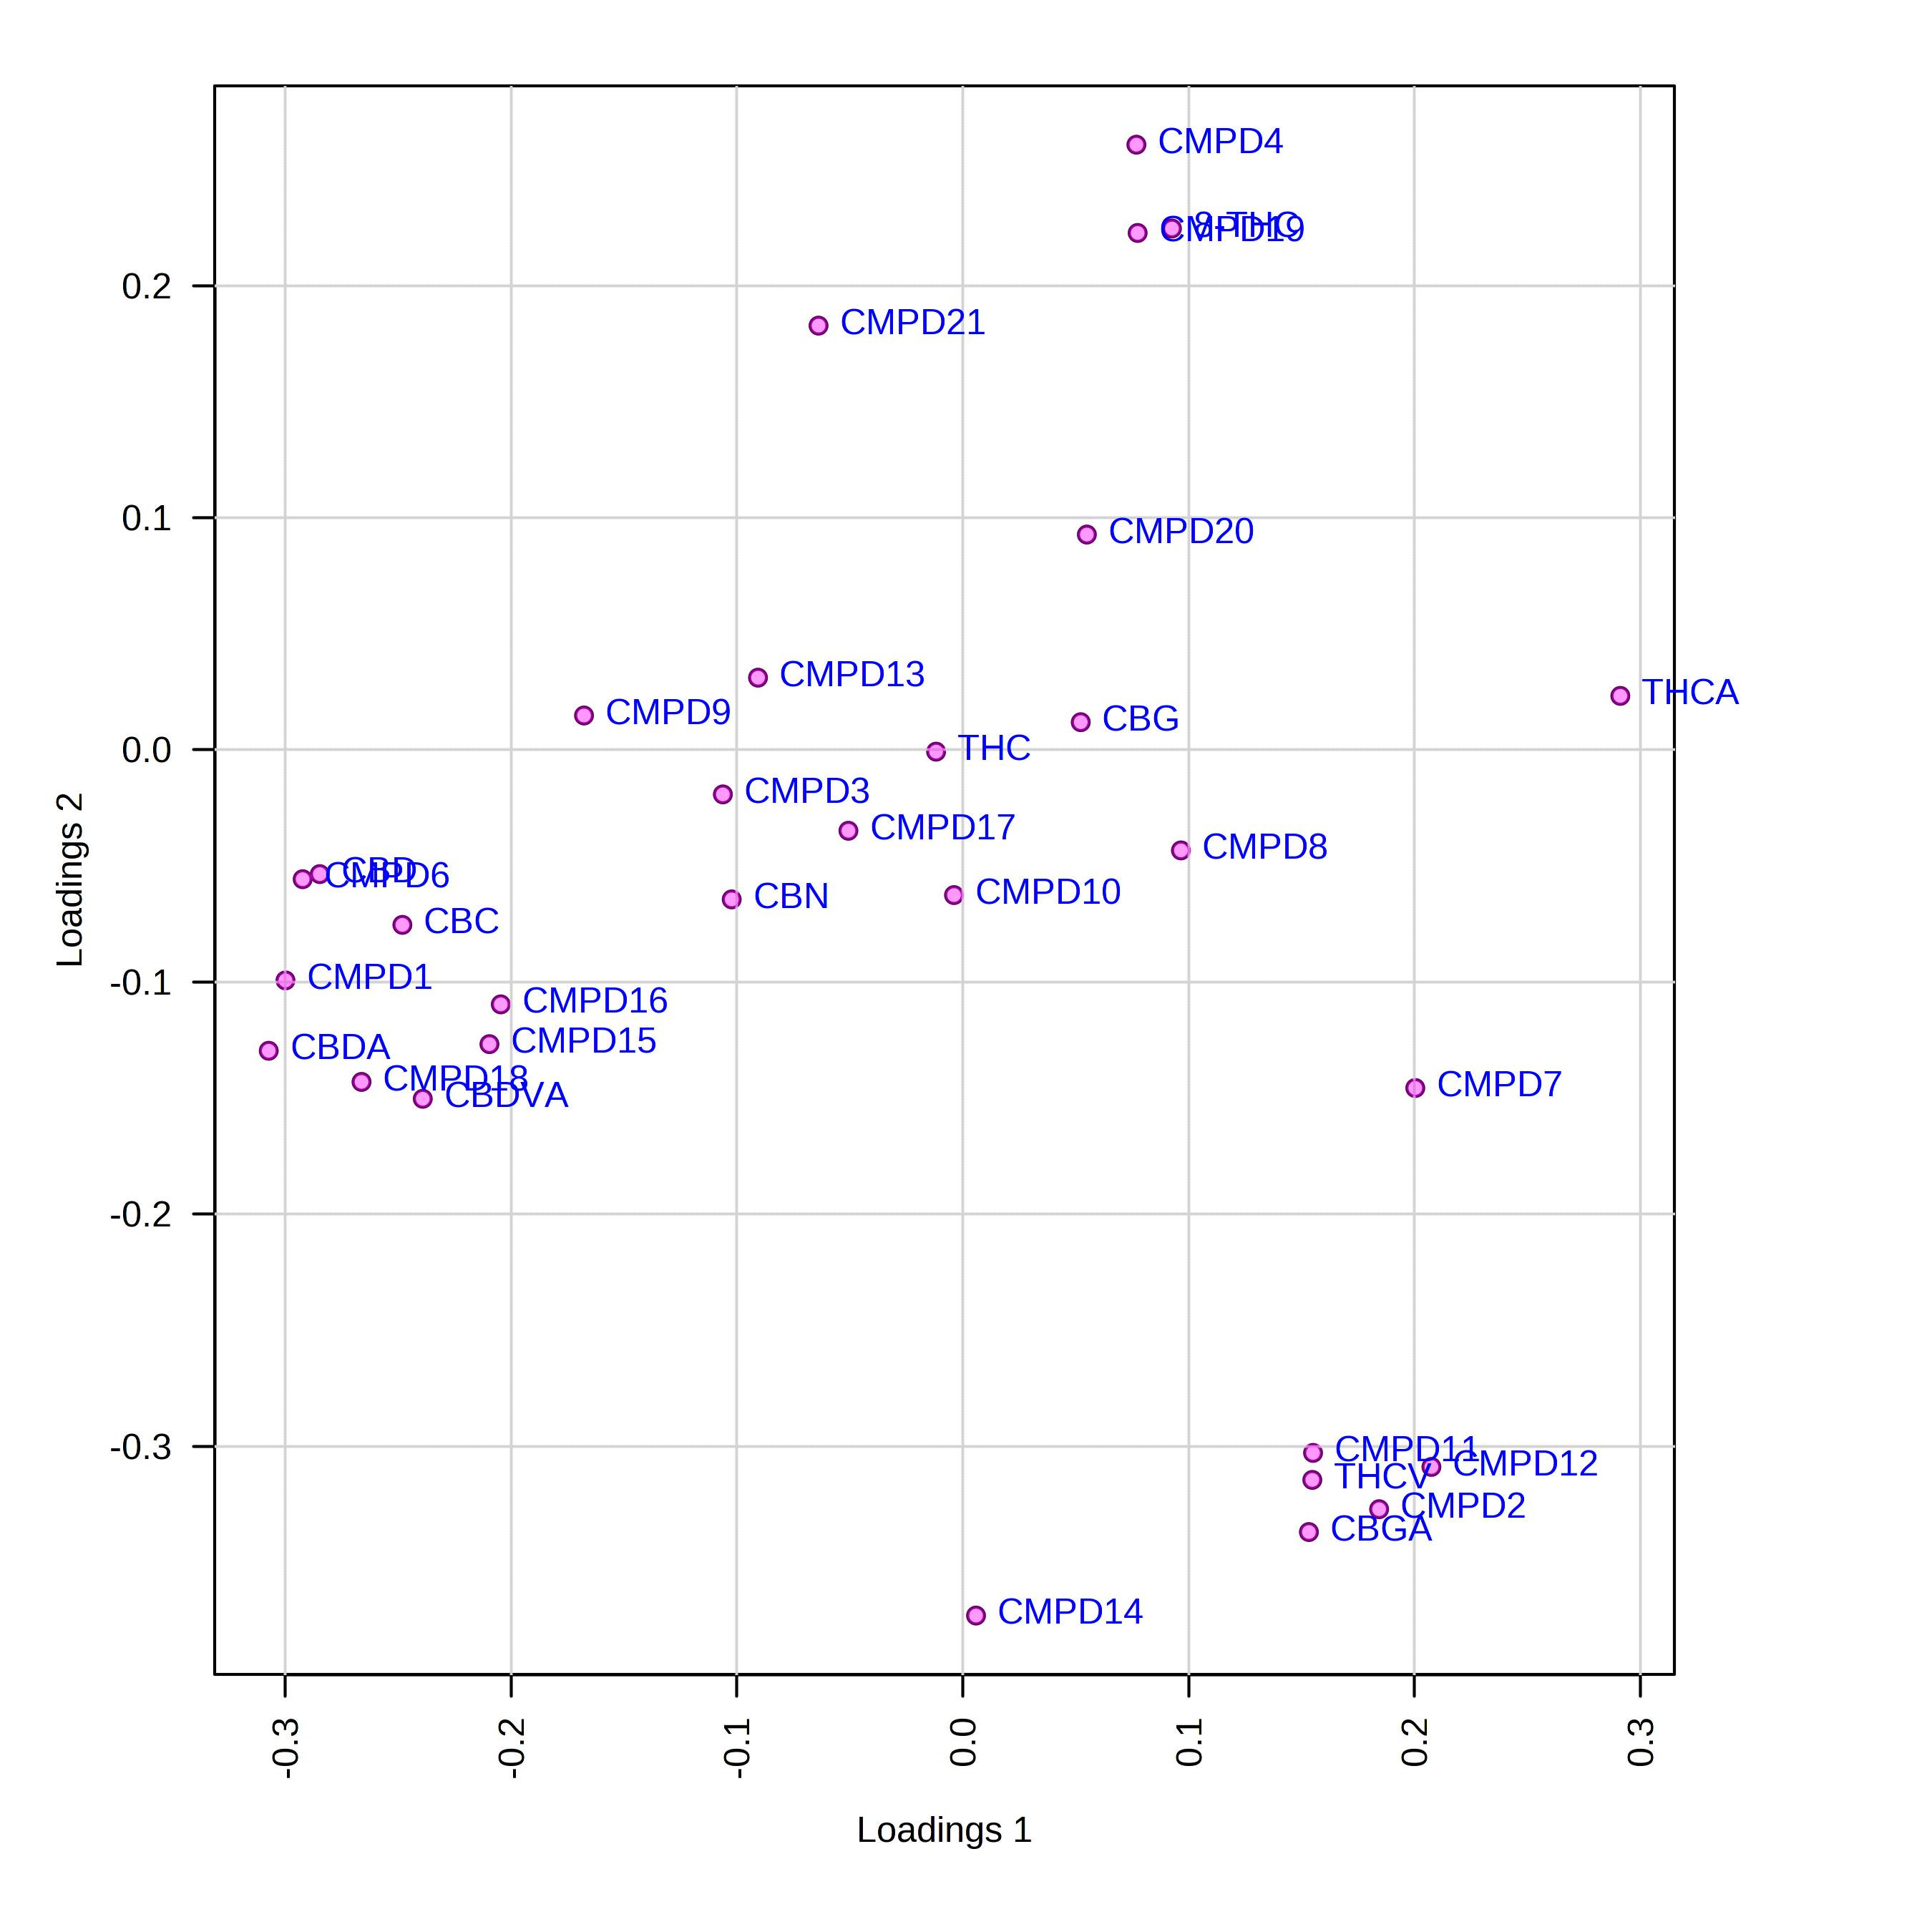
\includegraphics[width=0.7\textwidth]{pca_loading_0_dpi300.png}
\captionof{figure}{ PCA Loading Plot}
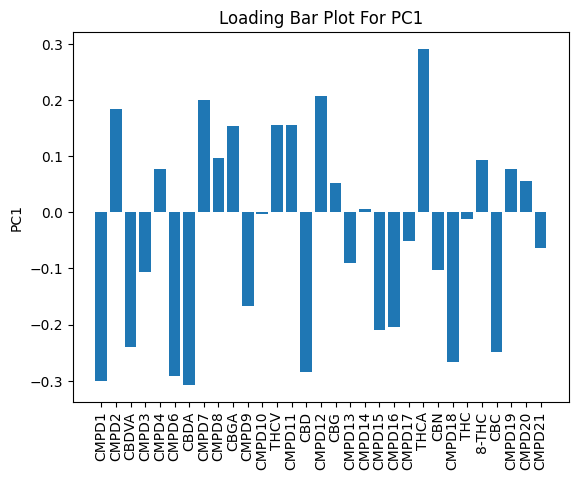
\includegraphics[width=0.7\textwidth]{PC1.png}
\captionof{figure}{}

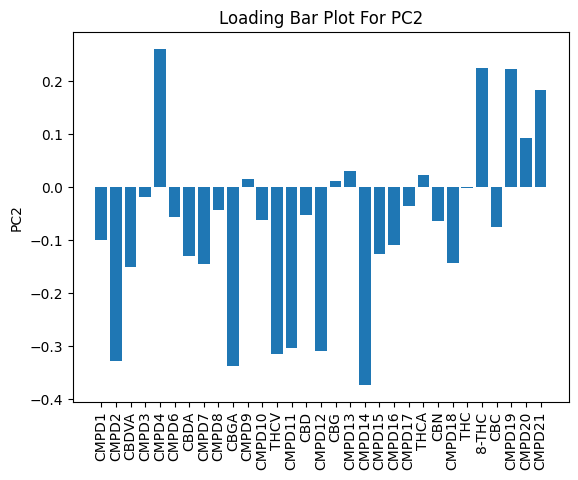
\includegraphics[width=0.7\textwidth]{PC2.png}
\captionof{figure}{}


\raggedright


We can see that THCA contributed a lot for loading 1 and CMPD4 (this is an unknown) contributed a lot for Loading 2. 

We compared that 

\section{Discussion}

\begin{thebibliography}{9}
\bibitem{Lab Manuel}
Adeyemi Adebowale, Julia Solonenka, Stephanie Bishop, Ian Cole, Abisola Kehinde, Elizabeth Mudge, and Susan Murch. ANALYTICAL  CHEMISTRY  LAB MANUAL.

\bibitem{dataset1}
Mudge, E.M.; Brown, P.N.; Murch, S.J. The Terroir of Cannabis: Terpene Metabolomics as a Tool
 to Understand Cannabis Selections. Planta Medica. 2019. DOI: 10.1055/a-0915-2550

\bibitem{dataset2}
Mudge, E.M.; Murch, S.J.; Brown, P.N. Chemometric analysis of cannabinoids: chemotaxonomy
 and domestication syndrome. Scientific Reports. 2018. 8, 13090. DOI:10.1038/s41598
 018-31120-2 1. 

 \bibitem{pandaCo}
“How to Create a Correlation Matrix using Pandas – Data to Fish.” https://datatofish.com/correlation-matrix-pandas/ (accessed Dec. 13, 2022).

\bibitem{PYPCA}
“sklearn.decomposition.PCA,” scikit-learn. https://scikit-learn/stable/modules/generated/sklearn.decomposition.PCA.html (accessed Dec. 13, 2022).
\bibitem{PCA}
C. Cheng, “Principal Component Analysis (PCA) Explained Visually with Zero Math,” Medium, Mar. 22, 2022. https://towardsdatascience.com/principal-component-analysis-pca-explained-visually-with-zero-math-1cbf392b9e7d (accessed Dec. 13, 2022).
\bibitem{info}
“A Mathematical Theory of Communication,” Harvard, The Bell System Technical Journal. [Online]. Available: https://people.math.harvard.edu/~ctm/home/text/others/shannon/entropy/entropy.pdf
\bibitem{SAM}
V. G. Tusher, R. Tibshirani, and G. Chu, “Significance analysis of microarrays applied to the ionizing radiation response,” Proc. Natl. Acad. Sci. U.S.A., vol. 98, no. 9, pp. 5116–5121, Apr. 2001, doi: 10.1073/pnas.091062498.


\bibitem{Market}
“North America Legal Cannabis Market Size Report, 2030.” https://www.grandviewresearch.com/industry-analysis/north-america-legal-cannabis-market-report (accessed Dec. 13, 2022).

\end{thebibliography}

\end{document}
